\part*{AbstractFS}
Est une librairie de fonctionnalité  permettant de réaliser des opérations de manipulation de système de fichier sur plusieurs différent support comme le FTP, le SSH ou les web-service.

Elle est implémenté en python en utilisant seulement les composant disponible dans la librairie standard, ce qui lui permet d'être utilisé sur n'importe quel système possédant python 2.6 – 2.7.

Son rôle est de permettre la création, la suppression de dossier ou les opérations de copie, déplacement de suppression de fichiers.

\section*{Structure}
La librairie est composée de plusieurs modules ayant chacun leur rôle:

\begin{itemize}
\item absException.py : contient les exception spécifique à la librairie
\item abstractFS.py : interface utilisateur de la librairie
\item base.py : module contenant la classe abstraite FS() d'où dériveront toutes les classe spécifique de manipulation de fichier, elle sert principalement au développeur pour lui permettre de déterminer les fonctionnalités qui lui reste à implémenter
\item ftp.py : module de système de fichier FTP, en utilisant la ftplib de la STL python
\item file.py : essentiellemnt un wrapper de la librairie os de la STL python.
\item ssh.py : non implémenté pour l'instant mais il le sera dans le futur.
\end{itemize}

\begin{figure}[h!]
	\centering
	\includegraphics[scale=0.35]{images/package_abstract_fs.png}
	\caption{Package AbstractFS}
\end{figure}

\section*{Fonctionnement de la couche d'abstraction}
\subsection*{mode d'utilisation}
La librairie présente un objet fs qui est utilisé comme le serait os

\newpage

\subsection*{Les différentes interfaces publiques}
Les noms sont essentiellement calqués sur les noms de fonction des librairies shutils et os

\begin{itemize}
\item copy(src, dst) : copie un fichier source vers une destination
\item move(src, dst) : déplace un fichier source vers une destination
\item remove(path) : supprime un fichier
\item makedirs(path) : créer une aborescence
\item rmdirs(path, delete) : supprime une aborescence, si delete vaut true les fichiers sont supprimé, sinon si l'aborescence contient des fichiers une erreur est levée.
\item listdir(path) : liste les éléments contenu dans path
\item isFile(path) : vérifie si path est un fichier 
\end{itemize}

Ces méthodes sont les seuls disponibles à l'utilisateur.

\subsection*{Les méthodes privés}
\subsubsection*{\_get\_handler}
Cette méthode permet soit d'instancier une classe de manipulation de système de fichier soit de récupérer une instance, si celle-ci est disponible.

Tout d'abord on vérifie si un handler du type désiré est disponible dans la liste des handler déjà enregistrés. Si aucun handler ne correspond on en instancie un nouveau du type désiré.
Dans le cas où le handler du bon type est trouvé on utilise celui, afin de vérifier si les paramètres (utilisateur, mot de passe, adresse du serveur, etc...) sont correctement renseignés.
Si la configuration est correct, on compare les identifiants de chacun des handlers afin de vérifier si un handler possédant les même identifiants de connexion, n'existe pas déjà, évitant ainsi des doublons de conection FTP par exemple.
Si rien de concluant n'est trouvé, on instancie un nouvel handler.

\subsubsection*{\_instanciateNewHandler}
En utilsant le schéma de l'url, elle instancie la classe FS() du module nom\_schema\_url.py, grâce à la librairie importlib.
Par exemple, si l'url est ftp://host, la méthode va récupérer une instance de la classe FS() du module ftp.py
Il lui indique ensuite les différents identifiants de connexion. Si une erreur survient lors de la connexion de l'handler, une exception est levée.
Sinon celui-ci est renvoyé.


\subsection*{La classe Streaming}

Elle tient lieu de FIFO, et stocke les différent blocs d'information avant traitement.
La taille de la FIFO et la taille d'un bloc peut-être paramétrées.
	
\subsubsection*{La méthode add\_task()}
	
Permet de rajouter un bloc de donné supplémentaire dans le FIFO, si celle-ci est pleine, un timeout se déclenche et le déroulement du script est arrêté, si à la fin du timeout la FIFO est toujours pleine, une erreur est déclenchée.

\subsubsection*{La méthode read()}
Renvoie un bloc de données, si la FIFO est vide, un timeout se déclenche et le déroulement du script est arrêté, si à la fin du timeout la FIFO est toujours vide, une erreur est levée.

\newpage

\subsection*{Les méthodes move et copy}
Celles-ci sont différentes dans leurs conceptions par rapport aux autres méthodes de la classe AbstractFS, en effet ces méthodes manipulent des fichiers et dossiers situé sur des systèmes de fichiers différents, ce qui impose d'utiliser deux manipulateurs de fichiers, un pour la source et autre pour la destination:

Avant de faire quoique ce soit on vérifie que les dossiers de sources et de destination

\begin{minted}[linenos=true]{python}

streaming  = Streaming(FIFO_size, blocksize)

tget = Thread(target=handler_src.get, args=(src["path"], streaming, error_get))
tput = Thread(target=handler_dst.put, args=(dst["path"], streaming, error_put))

tget.start()
tput.start()

tput.join()
tget.join()

\end{minted}

On génère tout d'abord une FIFO, puis deux threads l'un lançant méthode get de la scr l'autre la méthode put de la destination, possédant une même référence sr une FIFO.
L'idée première était d'utiliser un objet de type Stream qui aurait fait le buffer entre la fonction get qui aurait stocké l'intégralité des données binaire dans le stream donc en RAM!!! Puis cette objet aurait été donné à la méthode put qui aurait écrit les données. 

Cette piste a vite été abandonnée pour des raisons évidente de consommation de mémoire 
Le choix c'est donc porté vers une structure producteur-consommateur, afin de réaliser un gain en performance d'utilisation mémoire. Or ceci à un coup en vitesse de transfert entre la source et la destinatination, qui j ele rappelle, peut-être situé entre de la boucle locale.Il a donc valut ajuster la taille des blocs et la taille de la FIFO afin d'obtenir les meilleurs performances possibles.

Ceci grâce à l'utilitaire cProfile de python qui permet de comptabiliser le temps passer dans les différentes méthodes d'un Thread.

\begin{figure}[h!]
	\centering
	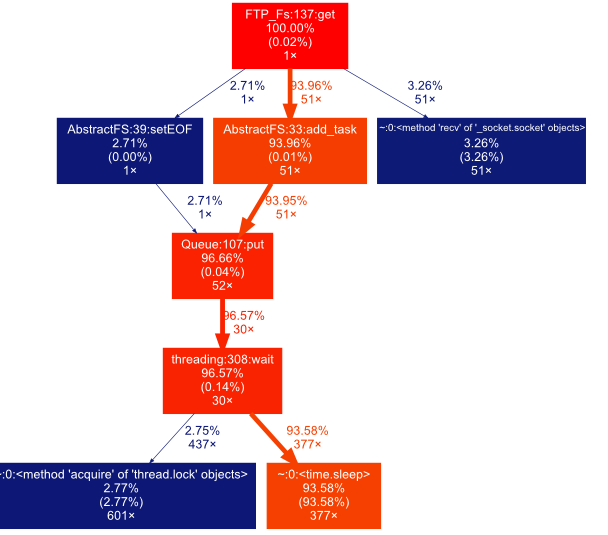
\includegraphics[scale=0.4]{images/without_optimization}
	\caption{Répartion du temps d'éxécution dans le cas d'une FIFO non optimisée}
\end{figure}

Nous remarquons ici que la méthode get passe énormément de temps à attendre la possibilité de pouvoir ajouter un bloc dans la file d'attente, ceci signifie que le consommateur (put), n'est pas assez rapide dans le dépilage (contrainte réseau, écriture sur le disque, etc...)

\begin{figure}[h!]
	\centering
	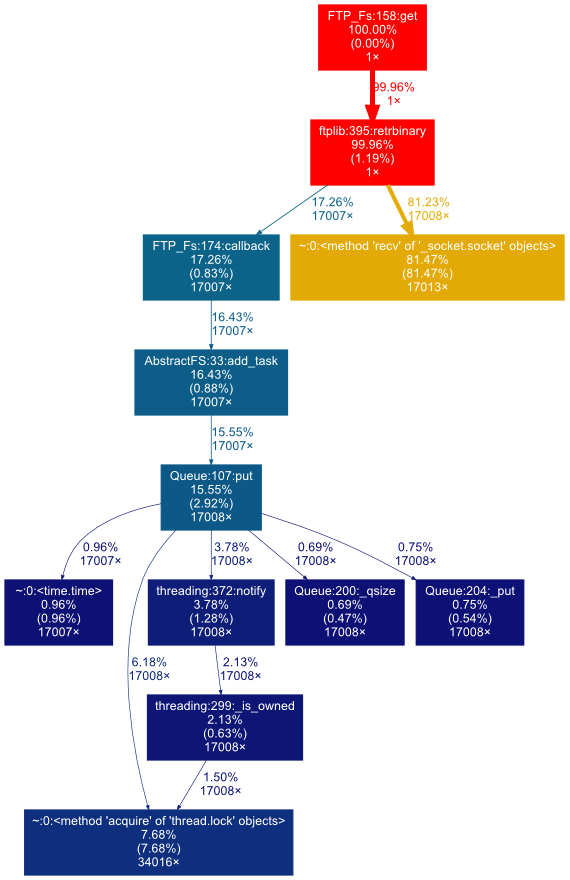
\includegraphics{images/with_optimization}
	\caption{Répartion du temps d'éxécution dans le cas d'une FIFO optimisée}
\end{figure}

Une fois les paramètres de la FIFO optimisée, la totalité du temps est consacrée à la lecture des données, ce qui est le fonctionnement voulu et attendu.